\documentclass[10pt, journal]{IEEEtran}

\usepackage[utf8]{inputenc}
\usepackage[T1]{fontenc}
\usepackage[english]{babel}
\usepackage{lmodern}
\usepackage{microtype}
\usepackage{amsmath, amssymb, amsthm, mathtools, bm}
\newtheorem{lemma}{Lemma}
\newtheorem{theorem}{Theorem}
\newtheorem{proposition}{Proposition}
\usepackage{siunitx}
\sisetup{locale = US, detect-all = true, exponent-product = \cdot}
\usepackage{booktabs, array, tabularx, multirow, makecell, colortbl}
\usepackage{graphicx}
\graphicspath{{figuras/}}
\usepackage{tikz}
\usetikzlibrary{arrows.meta, positioning, calc, shapes.geometric}
\usepackage{algorithm}
\usepackage{algpseudocode}
\usepackage{cite}
\usepackage{hyperref}
\hypersetup{colorlinks=true, linkcolor=blue, citecolor=blue, urlcolor=blue}

%% --- Paleta cromática institucional SENI-IA ---
\definecolor{seni-blue}{RGB}{0,45,98}
\definecolor{seni-red}{RGB}{206,17,38}
\definecolor{seni-gold}{RGB}{201,168,76}
\definecolor{seni-green}{RGB}{0,122,51}
\definecolor{seni-dark}{RGB}{26,26,26}

%% ====================================================================
%% CUADRO DE TÍTULOS SOBERANOS (4 OPCIONES CANÓNICAS EN PORTADA)
\title{SENI-142: An Open-Access Resilient Insular Transmission Benchmark of the Dominican Republic with Diakoptic Territorial Decomposition under Spatial Planning Law 368-22 --- Part~1: Network Architecture and Diakoptic HBCF Formulation}
\author{Junior~Alexis~Villanueva-Rosario,~\IEEEmembership{Ms.C., Ph.D.(c)}\\[0.3em]
{\normalsize\textnormal{\textbf{V-TECH} \textbar\ \textbf{V-CORE TECH S.R.L.} / \textbf{Villa-Core Technologies, S.L.}}}\\[0.15em]
{\footnotesize\textnormal{\textit{Department of Electrical Grids and Renewable Energy (EERR) Research}}}\\[0.15em]
{\footnotesize\textnormal{\textit{Doctoral Chair in Power Systems and Artificial Intelligence}}}\\[0.15em]
{\footnotesize\textnormal{Santo Domingo, Dominican Republic \textbar\ \texttt{ingjavillanueva@gmail.com}}}%
\thanks{J. A. Villanueva-Rosario is with the Department of Electrical Grids and Renewable Energy (EERR) Research, V-TECH (V-CORE TECH S.R.L. / Villa-Core Technologies, S.L.), Santo Domingo, Dominican Republic (e-mail: ingjavillanueva@gmail.com).}}

% --- Optimización de ubicación de figuras y tablas flotantes ---
\renewcommand{\topfraction}{0.95}
\renewcommand{\bottomfraction}{0.95}
\renewcommand{\textfraction}{0.05}
\renewcommand{\floatpagefraction}{0.8}
\renewcommand{\dbltopfraction}{0.95}
\renewcommand{\dblfloatpagefraction}{0.8}
\setcounter{topnumber}{4}
\setcounter{bottomnumber}{2}
\setcounter{totalnumber}{6}
\setcounter{dbltopnumber}{4}

\begin{document}
\maketitle
\begin{abstract}
This paper presents Part~I of SENI-142, an open, fully georeferenced benchmark of the complete bulk transmission system of the Dominican Republic. The physical infrastructure encompasses 171 fenced physical utility yards, reduced across spatial planning boundaries to 112 transmission-level substations (345/230/138~kV) and mapped into 142 nodal computation buses (115 bulk transmission buses and 27 condensed 69~kV boundary ports), with 135 transmission lines and 58 power transformers; the radial 69\,kV subtransmission layer is condensed into multiport equivalents preserving complex boundary injections and short-circuit impedances. The network is partitioned into ten planning regions aligned with national Law 368-22 and aggregated into four electrical macro-domains. A hierarchical boundary-coordinate formulation (HBCF) is applied, wherein the linear systems arising at each Newton--Raphson iteration are condensed exactly via the Schur complement, with an algebraic domain-decomposition residual of $\delta = 2.788 \times 10^{-14}$\,pu relative to a monolithic reference. Part~I states the graph representation, the equivalent reduction, the formal condensation proofs, the fail-closed digital-twin lifecycle, the OSB/OVB release architecture, the empirical data protocol, and the benchmark topology census, and defines the operator's own $N-1$ catalog of 215 contingencies under a two-layer reserve doctrine. The dataset, network parameters, and open validation harness are released through a public repository. The companion Part~II develops the multi-temporal multi-vector AC optimal power flow and reports the 87,360-state silicon campaign.
\end{abstract}

\begin{IEEEkeywords}
Benchmark testing, diakoptics, digital twins, insular power systems, power system resilience, Schur complement, spatial planning, transmission networks.
\end{IEEEkeywords}

% =========================================================================
% p1_sec01_introduction.tex — Part I Introduction (companion to Part II).
% Derived from the sealed monograph sec01; contributions C4/C5 routed to Part II.
% =========================================================================
\section{Introduction}
\label{sec:intro}

Insular interconnected systems occupy an extreme power engineering design space: lacking neighbor interconnections, every megawatt of reserve, reactive compensation, and damping capability must be produced within the same synchronous footprint that consumes it. The Dominican Republic is a canonical instance: a synchronous island of eleven million people without external ties, $>40\%$ of national load concentrated in the metropolitan Ozama region, an inertia anchor dominated by the Punta Catalina plant, and an instantaneous solar share reaching 36.6\% of demand in operational telemetry \cite{ocseni}. The national consequences of generation--load imbalance are evidenced by widespread service interruptions in November 2025 and February 2026 \cite{ocseni}, \cite{listin2025}, mobilizing emergency territorial response and renewing the debate on frequency stability, black-start readiness, and transmission observability \cite{blackout2004}. While the low-inertia dynamics of converter-dominated grids are theoretically established \cite{kundur1994}, \cite{tielens2016}, \cite{milano2018}, \cite{dorfler2013}, \cite{hatziargyriou2021}, empirical public instruments to analyze real insular systems remain primitive.

Power system benchmarks remain predominantly synthetic abstractions from the 1960s (WSCC 9-bus, IEEE 14-to-118-bus) with round academic reactances, fixed load triangles, and no real geography, climate, or maintenance histories. At the opposite pole, utility datasets remain encumbered by proprietary confidentiality, preventing independent re-execution. Open initiatives like MATPOWER \cite{matpower2011} and PGLib \cite{pglib2019} offer valuable instances, yet remain synthetic or anonymized. An open, complete, and measured model of an actual national transmission system with verifiable provenance represents an unmet public good for the insular Caribbean and the broader power systems community.

This article closes that gap with \textbf{SENI-142}, an open-access benchmark constructed around three commitments: (i) \textbf{Fidelity to measured reality}: a georeferenced CAD reconstruction of the Dominican bulk transmission estate validated against exactly 520 complete consecutive 168-hour weeks (87,360 hourly states spanning 3,640 Monday-to-Sunday days, 2016--2025 archive) dispatched unit-by-unit without interpolation. (ii) \textbf{Structural honesty about scale}: solving the complete national system via a hierarchical border-coordinate formulation (HBCF) in the diakoptic tradition \cite{kron1963}, \cite{happ1971}, condensed by the Schur complement \cite{zhang2005} and factorized across the ten territorial microgrids of the SNIT under Law 368-22, in harmony with General Electricity Law 125-01 \cite{ley368}. (iii) \textbf{Deterministic reproducibility}: a four-phase digital-twin lifecycle with fail-closed gates, detached SHA-512 manifests, and atomic kernel promotion guaranteeing bit-identical auditability.

The primary contributions are:
(i)~\textbf{C1 --- Benchmark:} An open, georeferenced model of the complete Dominican bulk network: 171 fenced physical utility yards, reduced to 112 transmission-level substations (345/230/138~kV) and mapped into 142 nodal computation buses (115 bulk + 27 condensed 69~kV ports), 135 transmission lines and 58 power transformers, released with topology, parameters, provenance metadata, and validation harness via GitHub.
(ii)~\textbf{C2 --- Formulation:} The HBCF diakoptic partition into ten territorial microgrids (Law 368-22) and four macro-subdomains with exact Schur condensation exhibiting complexity $O(\sum_k N_k^3 + N_B^3)$ versus monolithic $O(N^3)$ dense factorization.
(iii)~\textbf{C3 --- Deterministic digital twin:} A four-phase lifecycle (hermetic POSIX-namespace enclave with a 14-gate cascade; research-testbed static post-event $N-1$ verification against a 215-contingency catalog; SHA-512 Golden Master; and atomic kernel promotion via \texttt{renameat2} with zero regression) ensuring rigorous custodial reproducibility.
Contributions \textbf{C4} (multi-vector AC-OPF coupling hydrogen, 764~MW pumped hydro, and biomethanation) and \textbf{C5} (the 87,360-state campaign at 2.65~ms/state) are developed in the companion Part~II~\cite{seni142part2}.

The remainder of Part~I is organized as follows: Section~\ref{sec:methodology} presents the invariant formulation (graph model, 69~kV reduction, diakoptic HBCF, Schur proofs, and lifecycle); Section~\ref{sec:topology} details the 142-bus physical and microgrid topology; Section~\ref{sec:conclusion} concludes Part~I. The companion Part~II~\cite{seni142part2} develops the multi-vector AC-OPF, the 87,360-state campaign, severe contingencies, and policy implications.

% =========================================================================
% p1_sec02_diakoptic_hbcf.tex — Part I methodology core (diakoptic HBCF,
% Schur proofs, N-1 catalog, lifecycle, OSB/OVB, data protocol, clause).
% Extracted from sealed sec02 (post-rebase baseline 2026-10-21); OPF
% subsection routed to Part II; doctrines trimmed to the diakoptic set;
% tab:cuadro51 reduced to prose.
% =========================================================================
\section{Methodology: Diakoptic HBCF Schur Formulation and Fail-Closed Digital-Twin Lifecycle}
\label{sec:methodology}

The methodology is deliberately organized in two coupled components. The \textbf{invariant formulation} --- graph representation, equivalent reduction, spatial partition, exact condensation, data protocol, deterministic lifecycle, and regularization --- is problem-independent and transfers without modification across the family of studies built on this platform. The \textbf{territorial instantiation clause} binds this formulation to one reference reality: the national grid of the Dominican Republic, partitioned according to the country's own spatial planning statute. The subsections below follow that formulation through the numerical pipeline. The multi-temporal AC-OPF and the multi-vector flexibility layer are developed in the companion Part~II~\cite{seni142part2}.

\subsection{Steady-State AC Feasibility Scope}
\label{sub:scope}

SENI-142 is strictly a steady-state AC feasibility benchmark: each solved state is an algebraic equilibrium $F(\mathbf{x})=\mathbf{0}$ on the transmission grid. Fast electromagnetic transients (EMT), frequency dynamics, synthetic inertia, rate of change of frequency (RoCoF), and under-frequency load shedding (UFLS) are excluded. The outage of the largest generation block, Punta Catalina (752~MW, $\approx 21.8\%$ of the 3,450~MW reference national peak demand), is evaluated solely via steady-state voltage margins and post-contingency thermal branch solvability under co-optimized operating reserve; in the dynamic plane it is a frequency-stability event outside the static scope of this article.

\subsection{Sealed intake, physical census, and normative screen}
\label{sub:intake}

The solver accepts only a sealed input manifest verified before instantiation. In measured-estate mode, prospective assets outside commercial operation are excluded, ensuring the baseline represents the grid as operated. The physical census encompasses 171 fenced substations and 205 physical busbars (6 at 345~kV, 3 at 230~kV, 106 at 138~kV, and 90 at 69~kV) across 482 unreduced drawing branches, which condense to the 135 lines and 58 power transformers of the compute model.

Before admittance assembly, a normative screen validates all records against IEEE Std C37.2 \cite{ieeec37_2} bay arity, commercial equipment catalogs (ACSR/AAAC conductors, power transformers, reactive banks up to 250~MVAr), and IEC 61970 (CIM) standards \cite{iec61970}. Series reactances must satisfy $X > 0$, shunt susceptances $B \ge 0$, and thermal ratings $I_{\max} > 0$; any violation aborts execution fail-closed without synthetic default repairs.

\subsection{Columnar persistence and merit-order dispatch}
\label{sub:columnar}

Validated records are laid out as contiguous in-memory columns so that one instruction stream operates across nodal vectors without relational overhead. On those columns the thermal fleet is sorted by heat-rate merit, and each hour supplies the nodal demand pair $(P_d, Q_d)$.

\subsection{Graph-theoretic representation of the bulk network}
\label{sub:graph}

The bulk transmission system is modeled as a connected graph $\mathcal{G} = (\mathcal{V}, \mathcal{E})$ \cite{newman2010}, with $|\mathcal{V}| = 142$ nodal buses and branch set $\mathcal{E} = \mathcal{E}_{\mathrm{line}} \cup \mathcal{E}_{\mathrm{trafo}}$ ($|\mathcal{E}_{\mathrm{line}}| = 135$ lines, $|\mathcal{E}_{\mathrm{trafo}}| = 58$ transformers). On a 100~MVA base, the nodal admittance matrix $\mathbf{Y}_{\mathrm{bus}} \in \mathbb{C}^{142 \times 142}$ encodes 20,164 complex entries. Nodal complex power injections follow
\begin{equation}
S_i = P_i + jQ_i = V_i \sum_{j \in \mathcal{V}} Y_{ij}^{*}\, V_j^{*}, \qquad i \in \mathcal{V},
\label{eq:balance}
\end{equation}
with standard slack, PV, and PQ bus classifications \cite{tinney1967}. The angle reference is the JSAURI 345~kV bus ($V = 1.02\ \mathrm{pu}$) with bounded slack power \eqref{eq:slackbox}. Multi-voltage substations are modeled with distinct Kirchhoff buses coupled via transformer branches, mapping 112 transmission substations to 142 compute nodes (Section~\ref{sub:substations}).

Because branches are passive bilateral elements with conductances $g_{ij} > 0$, the admittance matrix is complex symmetric but intrinsically non-Hermitian:
\begin{equation}
\mathbf{Y}_{\mathrm{bus}}^{\mathsf{T}} = \mathbf{Y}_{\mathrm{bus}} \;\ne\; \mathbf{Y}_{\mathrm{bus}}^{\mathsf{H}} = \overline{\mathbf{Y}_{\mathrm{bus}}}^{\,\mathsf{T}},
\label{eq:nonhermitian}
\end{equation}
with maximum entry $\max_{i,j}\bigl|[\mathbf{Y}_{\mathrm{bus}} - \mathbf{Y}_{\mathrm{bus}}^{\mathsf{H}}]_{ij}\bigr| = 1{,}638.34$ on the 100~MVA base. All factorizations operate in complex symmetric arithmetic without assuming Hermitian structure, an invariant preserved under the Schur condensation of Section~\ref{sub:schur}. Figure~\ref{fig:topologia142} maps the 142 solved nodes (115 bulk yards at 345/230/138~kV and 27 retained 69~kV boundary ports) across the four Law 368-22 macrodomains ($\Omega_1$--$\Omega_4$).

% Full-page schematic of the 142-node trunk.
% 115 named bulk yards plus 27 retained 69 kV boundary terminals.
% Panel schematic. Raw drawing coordinates are not printed.

\begin{figure*}[!p]
\centering
\resizebox{\textwidth}{0.80\textheight}{%
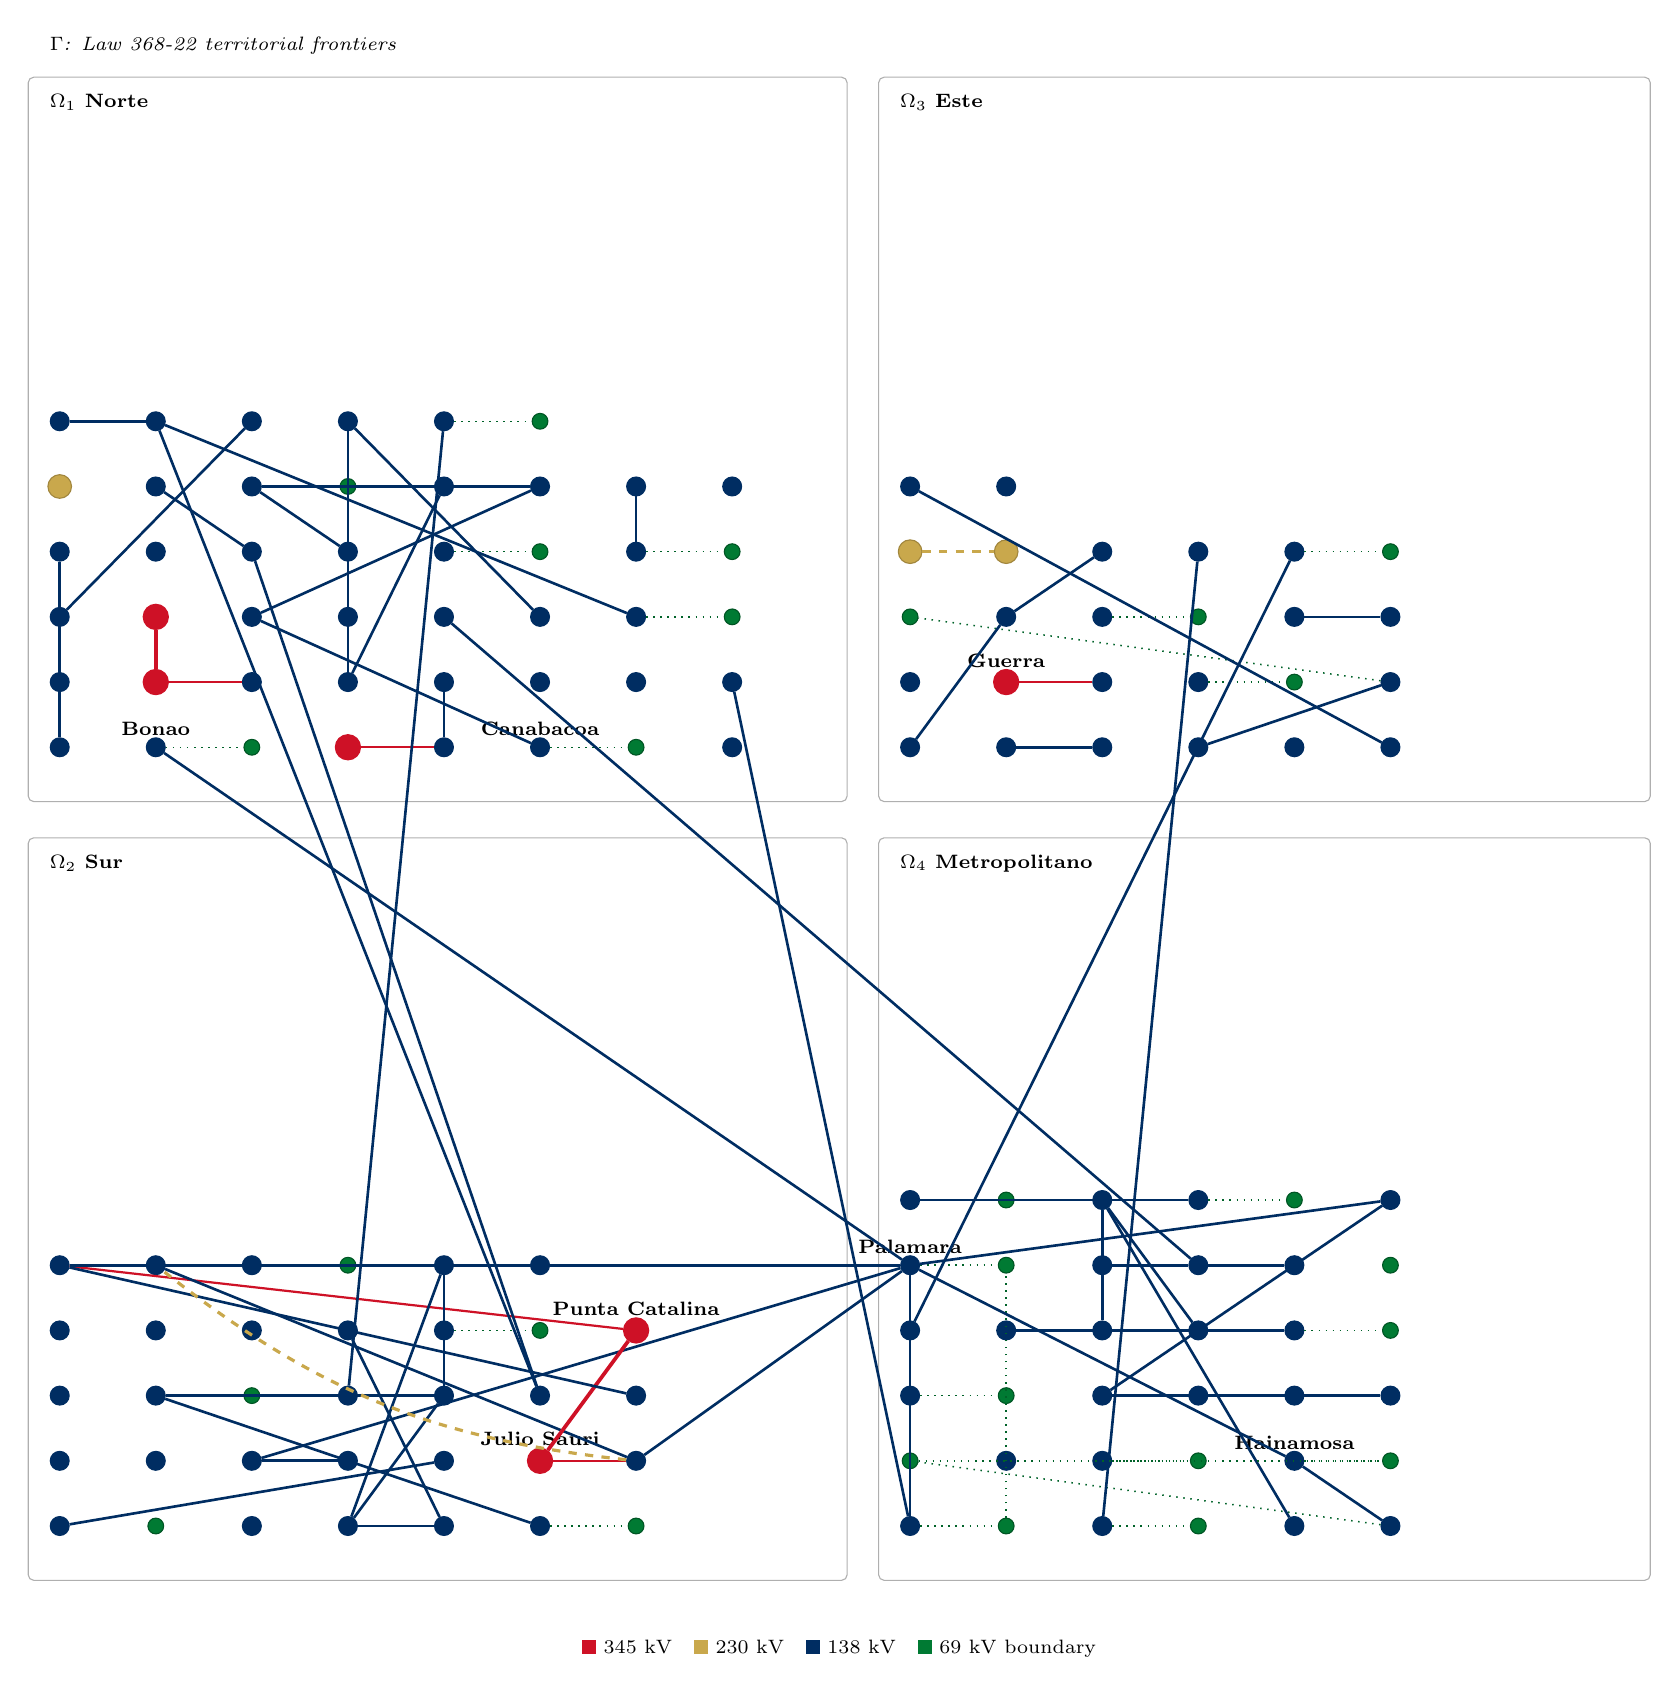
\begin{tikzpicture}[x=1cm,y=1.15cm,
  bus345/.style={circle, fill=seni-red, draw=seni-red, inner sep=0pt, minimum size=3.2mm},
  bus230/.style={circle, fill=seni-gold, draw=seni-gold!80!black, inner sep=0pt, minimum size=3.0mm},
  bus138/.style={circle, fill=seni-blue, draw=seni-blue, inner sep=0pt, minimum size=2.4mm},
  bus69/.style={circle, fill=seni-green, draw=seni-green!70!black, inner sep=0pt, minimum size=2.0mm},
  trunk345/.style={line width=1.35pt, seni-red},
  trunk230/.style={line width=1.15pt, seni-gold, dashed},
  trunk138/.style={line width=0.95pt, seni-blue},
  tie345/.style={line width=0.8pt, seni-red},
  tie230/.style={line width=0.75pt, seni-gold},
  tie138/.style={line width=0.6pt, seni-blue!70},
  tie69/.style={line width=0.55pt, seni-green!80!black, dotted}
]
\draw (0.15,16.95) node[anchor=west, font=\scriptsize\itshape] {$\Gamma$: Law 368-22 territorial frontiers};
\draw (10.3,-0.55) node[anchor=north, font=\scriptsize] {{\color{seni-red}\rule{5pt}{5pt}}~345~kV\quad {\color{seni-gold}\rule{5pt}{5pt}}~230~kV\quad {\color{seni-blue}\rule{5pt}{5pt}}~138~kV\quad {\color{seni-green}\rule{5pt}{5pt}}~69~kV boundary};
\draw[rounded corners=2pt, draw=seni-dark!35] (0.0,8.6) rectangle (10.4,16.6);
\draw (0.15,16.32) node[anchor=west, font=\bfseries\scriptsize] {$\Omega_1$ Norte};
\draw[rounded corners=2pt, draw=seni-dark!35] (10.8,8.6) rectangle (20.6,16.6);
\draw (10.95,16.32) node[anchor=west, font=\bfseries\scriptsize] {$\Omega_3$ Este};
\draw[rounded corners=2pt, draw=seni-dark!35] (0.0,0.0) rectangle (10.4,8.2);
\draw (0.15,7.92) node[anchor=west, font=\bfseries\scriptsize] {$\Omega_2$ Sur};
\draw[rounded corners=2pt, draw=seni-dark!35] (10.8,0.0) rectangle (20.6,8.2);
\draw (10.95,7.92) node[anchor=west, font=\bfseries\scriptsize] {$\Omega_4$ Metropolitano};
\node[bus345] (bBONAO3345) at (4.06,9.2) {};
\node[bus345] (bELNARANJO345) at (1.62,9.92) {};
\node[bus345, label={[font=\scriptsize\bfseries, inner sep=0.4pt]above:Guerra}] (bGUERRA345) at (12.42,9.92) {};
\node[bus345, label={[font=\scriptsize\bfseries, inner sep=0.4pt]above:Julio Sauri}] (bJULIOSAURI345) at (6.5,1.32) {};
\node[bus345] (bMANZANILLOPOWERLAND345) at (1.62,10.64) {};
\node[bus345, label={[font=\scriptsize\bfseries, inner sep=0.4pt]above:Punta Catalina}] (bPUNTACATALINA345) at (7.72,2.76) {};
\node[bus230] (bPVDC230) at (0.4,12.08) {};
\node[bus230] (bQUISQUEYA1230) at (11.2,11.36) {};
\node[bus230] (bQUISQUEYA2230) at (12.42,11.36) {};
\node[bus138] (bSPM138) at (16.08,11.36) {};
\node[bus138] (bSPM2138) at (11.2,12.08) {};
\node[bus138] (bAGUACLARA138) at (0.4,9.2) {};
\node[bus138] (bAGUACATE138) at (0.4,0.6) {};
\node[bus138] (bARROYOHONDO138) at (11.2,0.6) {};
\node[bus138] (bBARAHONACARBON138) at (2.84,0.6) {};
\node[bus138] (bBAYASOL138) at (4.06,0.6) {};
\node[bus138] (bBOCACHICA138) at (13.64,0.6) {};
\node[bus138, label={[font=\scriptsize\bfseries, inner sep=0.4pt]above:Bonao}] (bBONAO2138) at (1.62,9.2) {};
\node[bus138] (bBONAO3138) at (5.28,9.2) {};
\node[bus138] (bCALABAZA138) at (5.28,0.6) {};
\node[bus138, label={[font=\scriptsize\bfseries, inner sep=0.4pt]above:Canabacoa}] (bCANABACOA138) at (6.5,9.2) {};
\node[bus138] (bCIPLALUISA138) at (11.2,9.2) {};
\node[bus138] (bCNP138) at (16.08,0.6) {};
\node[bus138] (bCOASTAL138) at (12.42,9.2) {};
\node[bus138] (bCOTOPERI138) at (8.94,9.2) {};
\node[bus138] (bCRUCEDECABRAL2138) at (6.5,0.6) {};
\node[bus138] (bCUMAYASA138) at (13.64,9.2) {};
\node[bus138] (bDAJABON138) at (0.4,9.92) {};
\node[bus138] (bDAJAO138) at (17.3,0.6) {};
\node[bus138] (bELBRISAL138) at (0.4,1.32) {};
\node[bus138] (bELNARANJO138) at (2.84,9.92) {};
\node[bus138] (bELSEIBO138) at (14.86,9.2) {};
\node[bus138] (bELSOCO138) at (16.08,9.2) {};
\node[bus138] (bEMBAJADOR138) at (12.42,1.32) {};
\node[bus138] (bENERGAS4138) at (17.3,9.2) {};
\node[bus138] (bESPERANZA138) at (4.06,9.92) {};
\node[bus138] (bFALCONDO138) at (5.28,9.92) {};
\node[bus138] (bGIRASOL138) at (11.2,9.92) {};
\node[bus138] (bGUANILLO138) at (6.5,9.92) {};
\node[bus138] (bGUAYUBIN138) at (7.72,9.92) {};
\node[bus138] (bGUERRA138) at (13.64,9.92) {};
\node[bus138] (bGUZMANCITO138) at (1.62,1.32) {};
\node[bus138] (bHAINA138) at (13.64,1.32) {};
\node[bus138, label={[font=\scriptsize\bfseries, inner sep=0.4pt]above:Hainamosa}] (bHAINAMOSA138) at (16.08,1.32) {};
\node[bus138] (bHATOMAYOR2138) at (14.86,9.92) {};
\node[bus138] (bHERRERA138) at (11.2,2.04) {};
\node[bus138] (bHIGUEY138) at (17.3,9.92) {};
\node[bus138] (bITABO138) at (2.84,1.32) {};
\node[bus138] (bITABOTG138) at (4.06,1.32) {};
\node[bus138] (bJIGUEY138) at (5.28,1.32) {};
\node[bus138] (bJIMANI138) at (0.4,2.04) {};
\node[bus138] (bJUANDOLIO138) at (12.42,10.64) {};
\node[bus138] (bJULIOSAURI138) at (7.72,1.32) {};
\node[bus138] (bKM15DEAZUA138) at (1.62,2.04) {};
\node[bus138] (bLAGALLERA138) at (4.06,2.04) {};
\node[bus138] (bLAISABELA138) at (8.94,9.92) {};
\node[bus138] (bLAROMANA138) at (13.64,10.64) {};
\node[bus138] (bLOPEZANGOSTURA138) at (0.4,10.64) {};
\node[bus138] (bLOSMINA138) at (13.64,2.04) {};
\node[bus138] (bLOSMINA5138) at (14.86,2.04) {};
\node[bus138] (bLOSMINA6138) at (16.08,2.04) {};
\node[bus138] (bLOSMINA7138) at (17.3,2.04) {};
\node[bus138] (bLOSORIGENES138) at (11.2,2.76) {};
\node[bus138] (bLOSPRADOS138) at (12.42,2.76) {};
\node[bus138] (bMATADEPALMA2138) at (16.08,10.64) {};
\node[bus138] (bMATADERO138) at (13.64,2.76) {};
\node[bus138] (bMATAFONGO138) at (5.28,2.04) {};
\node[bus138] (bMATRISOL138) at (6.5,2.04) {};
\node[bus138] (bMETALDOM138) at (14.86,2.76) {};
\node[bus138] (bMETROPOLITANO138) at (16.08,2.76) {};
\node[bus138] (bMIRASOL138) at (17.3,10.64) {};
\node[bus138] (bMOCA138) at (2.84,10.64) {};
\node[bus138] (bMONCION138) at (6.5,10.64) {};
\node[bus138] (bMONTECRISTI138) at (4.06,10.64) {};
\node[bus138] (bMONTERIO138) at (5.28,10.64) {};
\node[bus138] (bNAGUA2138) at (7.72,10.64) {};
\node[bus138] (bNAVARRETE2138) at (0.4,11.36) {};
\node[bus138] (bNIBAJE138) at (1.62,11.36) {};
\node[bus138, label={[font=\scriptsize\bfseries, inner sep=0.4pt]above:Palamara}] (bPALAMARA138) at (11.2,3.48) {};
\node[bus138] (bPALENQUE138) at (7.72,2.04) {};
\node[bus138] (bPALOMINO138) at (0.4,2.76) {};
\node[bus138] (bPARAISO138) at (1.62,2.76) {};
\node[bus138] (bPAYITA138) at (2.84,11.36) {};
\node[bus138] (bPEDERNALES138) at (2.84,2.76) {};
\node[bus138] (bPERAVIA138) at (4.06,2.76) {};
\node[bus138] (bPIMENTEL138) at (4.06,11.36) {};
\node[bus138] (bPIZARRETE138) at (5.28,2.76) {};
\node[bus138] (bPLAYADORADA138) at (5.28,11.36) {};
\node[bus138] (bPOWERSHIPKPS01138) at (13.64,3.48) {};
\node[bus138] (bPOWERSHIPKPS26138) at (14.86,3.48) {};
\node[bus138] (bPOWERSHIPKPS60138) at (16.08,3.48) {};
\node[bus138] (bPUERTOPLATA2138) at (7.72,11.36) {};
\node[bus138] (bPUNTACATALINA138) at (0.4,3.48) {};
\node[bus138] (bRIOSANJUAN138) at (1.62,12.08) {};
\node[bus138] (bSFM138) at (2.84,12.08) {};
\node[bus138] (bSAJOMA138) at (5.28,12.08) {};
\node[bus138] (bSALCEDO138) at (6.5,12.08) {};
\node[bus138] (bSAMANA138) at (0.4,12.8) {};
\node[bus138] (bSANCRISTOBALNORTE138) at (1.62,3.48) {};
\node[bus138] (bSANFELIPE138) at (7.72,12.08) {};
\node[bus138] (bSANJUAN2138) at (2.84,3.48) {};
\node[bus138] (bSANPEDROBIOENERGY138) at (13.64,11.36) {};
\node[bus138] (bSANCHEZ138) at (1.62,12.8) {};
\node[bus138] (bSANTANASOL138) at (5.28,3.48) {};
\node[bus138] (bSANTIAGORODRIGUEZ138) at (8.94,12.08) {};
\node[bus138] (bSIBA138) at (14.86,11.36) {};
\node[bus138] (bSULTANADELESTE138) at (12.42,12.08) {};
\node[bus138] (bTAVERA138) at (2.84,12.8) {};
\node[bus138] (bTIMBEQUE2138) at (11.2,4.2) {};
\node[bus138] (bUASD138) at (13.64,4.2) {};
\node[bus138] (bVALDESIA138) at (6.5,3.48) {};
\node[bus138] (bVALVERDEMAO138) at (4.06,12.8) {};
\node[bus138] (bVILLADUARTE138) at (14.86,4.2) {};
\node[bus138] (bVILLAMELLA138) at (17.3,4.2) {};
\node[bus138] (bZFSANTIAGO138) at (5.28,12.8) {};
\node[bus69] (bARROYOHONDO69) at (12.42,0.6) {};
\node[bus69] (bBARAHONA69) at (1.62,0.6) {};
\node[bus69] (bBOCACHICA69) at (14.86,0.6) {};
\node[bus69] (bBONAO269) at (2.84,9.2) {};
\node[bus69] (bCANABACOA69) at (7.72,9.2) {};
\node[bus69] (bCRUCEDECABRAL269) at (7.72,0.6) {};
\node[bus69] (bDAJAO69) at (11.2,1.32) {};
\node[bus69] (bHAINA69) at (14.86,1.32) {};
\node[bus69] (bHAINAMOSA69) at (17.3,1.32) {};
\node[bus69] (bHATOMAYOR269) at (16.08,9.92) {};
\node[bus69] (bHERRERA69) at (12.42,2.04) {};
\node[bus69] (bHIGUEY69) at (11.2,10.64) {};
\node[bus69] (bKM15DEAZUA69) at (2.84,2.04) {};
\node[bus69] (bMETROPOLITANO69) at (17.3,2.76) {};
\node[bus69] (bNAGUA269) at (8.94,10.64) {};
\node[bus69] (bPALAMARA69) at (12.42,3.48) {};
\node[bus69] (bPIZARRETE69) at (6.5,2.76) {};
\node[bus69] (bPLAYADORADA69) at (6.5,11.36) {};
\node[bus69] (bPUERTOPLATA269) at (8.94,11.36) {};
\node[bus69] (bLAROMANA69) at (14.86,10.64) {};
\node[bus69] (bSANJUAN269) at (4.06,3.48) {};
\node[bus69] (bSFM69) at (4.06,12.08) {};
\node[bus69] (bSPM69) at (17.3,11.36) {};
\node[bus69] (bTIMBEQUE69) at (17.3,3.48) {};
\node[bus69] (bTIMBEQUE269) at (12.42,4.2) {};
\node[bus69] (bVILLADUARTE69) at (16.08,4.2) {};
\node[bus69] (bZFSANTIAGO69) at (6.5,12.8) {};
\draw[tie345] (bBONAO3345) -- (bBONAO3138);
\draw[tie345] (bELNARANJO345) -- (bELNARANJO138);
\draw[tie345] (bGUERRA345) -- (bGUERRA138);
\draw[tie345] (bJULIOSAURI345) -- (bJULIOSAURI138);
\draw[tie345] (bPUNTACATALINA345) -- (bPUNTACATALINA138);
\draw[tie69] (bSPM138) -- (bSPM69);
\draw[tie69] (bARROYOHONDO138) -- (bARROYOHONDO69);
\draw[tie69] (bBOCACHICA138) -- (bBOCACHICA69);
\draw[tie69] (bBONAO2138) -- (bBONAO269);
\draw[tie69] (bCANABACOA138) -- (bCANABACOA69);
\draw[tie69] (bCRUCEDECABRAL2138) -- (bCRUCEDECABRAL269);
\draw[tie69] (bDAJAO138) -- (bDAJAO69);
\draw[tie69] (bHAINA138) -- (bHAINA69);
\draw[tie69] (bHAINAMOSA138) -- (bHAINAMOSA69);
\draw[tie69] (bHATOMAYOR2138) -- (bHATOMAYOR269);
\draw[tie69] (bHERRERA138) -- (bHERRERA69);
\draw[tie69] (bHIGUEY138) -- (bHIGUEY69);
\draw[tie69] (bKM15DEAZUA138) -- (bKM15DEAZUA69);
\draw[tie69] (bLAROMANA138) -- (bLAROMANA69);
\draw[tie69] (bMETROPOLITANO138) -- (bMETROPOLITANO69);
\draw[tie69] (bNAGUA2138) -- (bNAGUA269);
\draw[tie69] (bPALAMARA138) -- (bPALAMARA69);
\draw[tie69] (bPIZARRETE138) -- (bPIZARRETE69);
\draw[tie69] (bPLAYADORADA138) -- (bPLAYADORADA69);
\draw[tie69] (bPUERTOPLATA2138) -- (bPUERTOPLATA269);
\draw[tie69] (bSFM138) -- (bSFM69);
\draw[tie69] (bSANJUAN2138) -- (bSANJUAN269);
\draw[tie69] (bTIMBEQUE2138) -- (bTIMBEQUE269);
\draw[tie69] (bVILLADUARTE138) -- (bVILLADUARTE69);
\draw[tie69] (bZFSANTIAGO138) -- (bZFSANTIAGO69);
\draw[trunk138] (bAGUACLARA138) -- (bNAVARRETE2138);
\draw[trunk138] (bAGUACATE138) -- (bJIGUEY138);
\draw[tie69] (bARROYOHONDO69) -- (bPALAMARA69);
\draw[trunk138] (bARROYOHONDO138) -- (bLAISABELA138);
\draw[trunk138] (bARROYOHONDO138) -- (bPALAMARA138);
\draw[trunk138] (bBAYASOL138) -- (bCALABAZA138);
\draw[trunk138] (bBAYASOL138) -- (bMATAFONGO138);
\draw[trunk138] (bBAYASOL138) -- (bSANTANASOL138);
\draw[trunk138] (bBOCACHICA138) -- (bSIBA138);
\draw[trunk138] (bBONAO2138) -- (bPALAMARA138);
\draw[trunk138] (bBONAO3138) -- (bFALCONDO138);
\draw[trunk138] (bCALABAZA138) -- (bPERAVIA138);
\draw[trunk138] (bCANABACOA138) -- (bMOCA138);
\draw[trunk138] (bCIPLALUISA138) -- (bJUANDOLIO138);
\draw[trunk138] (bCNP138) -- (bUASD138);
\draw[trunk138] (bCOASTAL138) -- (bCUMAYASA138);
\draw[trunk138] (bCRUCEDECABRAL2138) -- (bKM15DEAZUA138);
\draw[tie69] (bDAJAO69) -- (bHAINAMOSA69);
\draw[trunk138] (bDAJAO138) -- (bHAINAMOSA138);
\draw[trunk345] (bELNARANJO345) -- (bMANZANILLOPOWERLAND345);
\draw[trunk138] (bELSEIBO138) -- (bHIGUEY138);
\draw[trunk138] (bENERGAS4138) -- (bSPM2138);
\draw[trunk138] (bESPERANZA138) -- (bSAJOMA138);
\draw[trunk138] (bESPERANZA138) -- (bVALVERDEMAO138);
\draw[trunk138] (bHAINAMOSA138) -- (bPALAMARA138);
\draw[trunk138] (bITABO138) -- (bITABOTG138);
\draw[trunk138] (bITABO138) -- (bPALAMARA138);
\draw[trunk138] (bJUANDOLIO138) -- (bSANPEDROBIOENERGY138);
\draw[trunk138] (bJULIOSAURI138) -- (bPALAMARA138);
\draw[trunk138] (bJULIOSAURI138) -- (bSANCRISTOBALNORTE138);
\draw[trunk345] (bJULIOSAURI345) -- (bPUNTACATALINA345);
\draw[trunk138] (bKM15DEAZUA138) -- (bMATAFONGO138);
\draw[trunk138] (bLAGALLERA138) -- (bZFSANTIAGO138);
\draw[trunk138] (bLOPEZANGOSTURA138) -- (bTAVERA138);
\draw[trunk138] (bLOSMINA138) -- (bLOSMINA5138);
\draw[trunk138] (bLOSMINA138) -- (bLOSMINA6138);
\draw[trunk138] (bLOSMINA138) -- (bLOSMINA7138);
\draw[trunk138] (bLOSMINA138) -- (bVILLAMELLA138);
\draw[trunk138] (bLOSMINA5138) -- (bLOSMINA6138);
\draw[trunk138] (bLOSMINA6138) -- (bLOSMINA7138);
\draw[trunk138] (bLOSORIGENES138) -- (bSPM138);
\draw[trunk138] (bLOSPRADOS138) -- (bMETROPOLITANO138);
\draw[trunk138] (bMATADEPALMA2138) -- (bMIRASOL138);
\draw[trunk138] (bMATADERO138) -- (bMETALDOM138);
\draw[trunk138] (bMATADERO138) -- (bUASD138);
\draw[trunk138] (bMATAFONGO138) -- (bPIZARRETE138);
\draw[trunk138] (bMATAFONGO138) -- (bSANTANASOL138);
\draw[trunk138] (bMATRISOL138) -- (bPAYITA138);
\draw[trunk138] (bMATRISOL138) -- (bSANCHEZ138);
\draw[trunk138] (bMETALDOM138) -- (bUASD138);
\draw[trunk138] (bMOCA138) -- (bSALCEDO138);
\draw[trunk138] (bMONCION138) -- (bVALVERDEMAO138);
\draw[trunk138] (bMONTERIO138) -- (bPOWERSHIPKPS26138);
\draw[trunk138] (bNAGUA2138) -- (bSANCHEZ138);
\draw[trunk138] (bPALAMARA138) -- (bSANCRISTOBALNORTE138);
\draw[trunk138] (bPALAMARA138) -- (bVALDESIA138);
\draw[trunk138] (bPALAMARA138) -- (bVILLAMELLA138);
\draw[trunk138] (bPALENQUE138) -- (bPUNTACATALINA138);
\draw[trunk138] (bPAYITA138) -- (bRIOSANJUAN138);
\draw[trunk138] (bPIMENTEL138) -- (bSFM138);
\draw[trunk138] (bPIZARRETE138) -- (bSANTANASOL138);
\draw[trunk138] (bPOWERSHIPKPS01138) -- (bPOWERSHIPKPS26138);
\draw[trunk138] (bPOWERSHIPKPS26138) -- (bPOWERSHIPKPS60138);
\draw[trunk138] (bPUERTOPLATA2138) -- (bSANFELIPE138);
\draw[trunk138] (bPUNTACATALINA138) -- (bVALDESIA138);
\draw[trunk230] (bQUISQUEYA1230) -- (bQUISQUEYA2230);
\draw[trunk138] (bSFM138) -- (bSALCEDO138);
\draw[trunk138] (bSAMANA138) -- (bSANCHEZ138);
\draw[trunk138] (bSANCRISTOBALNORTE138) -- (bVALDESIA138);
\draw[trunk138] (bTIMBEQUE2138) -- (bVILLADUARTE138);
\draw[trunk230] (bJULIOSAURI138) to[bend left=16] (bSANCRISTOBALNORTE138);
\end{tikzpicture}%
}
\caption{Schematic of the 142-node trunk, grouped into the four electrical macrodomains of Law 368-22 ($\Omega_1$ Norte, $\Omega_2$ Sur, $\Omega_3$ Este, $\Omega_4$ Metropolitano). Color is the measured nominal voltage: 345~kV in red, 230~kV in gold, 138~kV in blue, and the 27 retained 69~kV boundary terminals in green. A stroke joins two solved buses only: same-estate autotransformer links; yard records that name both ends, including the Palamara 138~kV bays to Julio Sauri, San Cristobal Norte, Hainamosa, Itabo, Valdesia, Bonao 2, Villa Mella and Arroyo Hondo; the 345~kV corridors Punta Catalina--Julio Sauri and Manzanillo Power Land--El Naranjo; the 138~kV link km~15 de Azua--Cruce de Cabral~2; the 230~kV tie Quisqueya~1--Quisqueya~2; and every other same-voltage pair whose colinear one-line trace arrives at a second census label. Parallel circuits are one stroke. The dashed bent stroke is the published 230~kV Julio Sauri--San Cristobal Norte reinforcement between the two 138~kV estates, because the census declares no separate 230~kV bus there. A record whose far terminal is not a census bus is omitted. Panel positions are schematic. Raw drawing coordinates are not shown.}
\label{fig:topologia142}
\end{figure*}


\subsection{Equivalent reduction of the 69 kV subtransmission layer}
\label{sub:reduction}

Sixty-three radial laterals of the ninety 69~kV busbars are condensed into static multiport equivalents of Th\'evenin/Norton type, while 27 boundary terminals remain solved buses at their measured 69~kV. Together with the 115 bulk nodes (at 345, 230, and 138~kV), the solved model totals $142 = 115 + 27$ buses. For each boundary port $p$ with condensed interior $\Omega_r$, the equivalent preserves hourly complex injections, short-circuit impedances $Z_{\mathrm{cc}}$ via Kron reduction, and internal losses $\Delta S_{\mathrm{loss}}$:
\begin{equation}
V_p = E_{\mathrm{th}}^{(r)} - Z_{\mathrm{th}}^{(r)} I_p, \qquad \sum_{i \in \Omega_r} S_i = V_p I_p^{*} + \Delta S_{\mathrm{loss}},
\label{eq:thevenin}
\end{equation}
consistent with IEEE Std 399 \cite{ieee399} and IEC 61970 (CIM) \cite{iec61970}. Eliminating high-$R/X$ laterals prevents Jacobian ill-conditioning and enables robust convergence. Synchronous units retain standard $P$--$Q$ capabilities, whereas inverter-interfaced renewable resources follow the continuous regularization of Section~\ref{sub:regularization}.

\subsection{Breadth-first scaling of connectivity}
\label{sub:bfs}

Let $\mathcal{G}_Y=(\mathcal{V},\mathcal{E}_Y)$ be the sparsity graph of $\mathbf{Y}_{\mathrm{bus}}$. Breadth-first search (BFS, denoted M09, Algorithm~\ref{alg:bfs}) starts at the Julio Sauri slack and traverses all reachable buses on $\mathcal{G}_Y$. Unvisited buses mark disconnected islands ($V_m=\mathrm{NaN}$); visited degree-one buses identify radial antennas candidate for 69~kV condensation (Section~\ref{sub:reduction}). The traversal places interior buses before border buses, providing the ordering for the HBCF Schur partition (Section~\ref{sub:hbcf}).

\begin{algorithm}[!t]
\caption{Breadth-first scaling on the admittance graph (M09)}
\label{alg:bfs}
\begin{algorithmic}[1]
\Require sparsity graph $\mathcal{G}_Y=(\mathcal{V},\mathcal{E}_Y)$, slack $s$
\State $Q \gets (s)$, $\mathrm{seen}\gets\{s\}$, $\pi\gets(s)$
\While{$Q\neq\emptyset$}
  \State $u \gets \mathrm{pop}(Q)$
  \For{$v\in\mathcal{N}(u)$}
    \If{$v\notin\mathrm{seen}$}
      \State $\mathrm{seen}\gets\mathrm{seen}\cup\{v\}$; append $v$ to $Q$ and to $\pi$
    \EndIf
  \EndFor
\EndWhile
\State $\mathcal{I}\gets\mathcal{V}\setminus\mathrm{seen}$ \Comment{islands, $V_m=\mathrm{NaN}$}
\State $\mathcal{A}\gets\{u\in\mathrm{seen}:\deg(u)=1\}$ \Comment{radial antennas}
\State \Return permutation $\pi$, islands $\mathcal{I}$, antennas $\mathcal{A}$
\end{algorithmic}
\end{algorithm}

The reordering forms a permutation $\mathbf{P}$ preserving singular values: $\kappa_2(\mathbf{P}\mathbf{J}\mathbf{P}^{\mathsf{T}})=\kappa_2(\mathbf{J})$. On the SENI base case, the measured movement reflects an operating-point shift between real and ideal networks:
\begin{equation}
\kappa_{\mathrm{real}} = 341.21, \quad
\kappa_{\mathrm{ideal}} = 365.91, \quad
\frac{\kappa_{\mathrm{ideal}}-\kappa_{\mathrm{real}}}{\kappa_{\mathrm{real}}} = +7.24\%,
\label{eq:bfs}
\end{equation}
tightening voltage margins and losses without expanding state dimension. IEEE Std 399 \cite{ieee399} provides industrial context rather than a rigid threshold on $\kappa(\mathbf{J})$.

\subsection{Centered reactive regularization and inverter capability}
\label{sub:regularization}

Hard PV--PQ bus switching at generator reactive limits induces limit cycles in Newton iterations. To ensure differentiability, generator and inverter reactive support follows a centered $C^1$ sigmoidal controller with $Q(V_{\mathrm{ref}})=0$:
\begin{equation}
Q_{\mathrm{sgen}}(V) = Q_{\max} \left( \frac{2}{1 + e^{-\gamma (V_{\mathrm{ref}} - V)}} - 1 \right),
\label{eq:qsgen}
\end{equation}
whose derivative $\partial Q / \partial V = -2\gamma Q_{\max}\sigma(1-\sigma)$ with $\sigma=(1+e^{-\gamma(V_{\mathrm{ref}}-V)})^{-1}$ enters $\mathbf{J}_{QV}$ without chatter (measured regularization error $5.32 \times 10^{-12}$). Inverter injections are bounded by the apparent-power disk
\begin{equation}
P_{g,t}^{2} + Q_{g,t}^{2} \le \bigl(S_{g}^{\max}\bigr)^{2},
\label{eq:capability}
\end{equation}
complying with IEEE Std 2800-2022 \cite{ieee2800} and IEEE Std 1547-2018 \cite{ieee1547}.

\subsection{Four-block Jacobian and the solver cascade}
\label{sub:jacobian}

The Newton iteration employs the full unreduced four-block polar Jacobian without decoupled approximations:
\begin{equation}
\mathbf{J} =
\begin{bmatrix}
\mathbf{J}_{P\theta} & \mathbf{J}_{PV} \\
\mathbf{J}_{Q\theta} & \mathbf{J}_{QV}
\end{bmatrix}
=
\begin{bmatrix}
\partial \mathbf{P} / \partial \boldsymbol{\theta} & \partial \mathbf{P} / \partial \mathbf{V} \\[3pt]
\partial \mathbf{Q} / \partial \boldsymbol{\theta} & \partial \mathbf{Q} / \partial \mathbf{V}
\end{bmatrix} \in \mathbb{R}^{282 \times 282},
\label{eq:polar_j}
\end{equation}
for the 141 non-slack buses. The solution cascade advances from a flat start through fast-decoupled estimation to polar Newton--Raphson (stopping tolerance $10^{-8}$~pu), falling back to damped Levenberg--Marquardt if ill-conditioning is encountered. Together with $\mathbf{Y}_{\mathrm{bus}} \in \mathbb{C}^{142 \times 142}$ (20,164 complex entries), $\mathbf{J}$ forms the sealed matrix pair audited under Section~\ref{sub:seals}.

\subsection{Multi-tier numerical verification}
\label{sub:trinity}

Each operating state is audited by three independent checks: the physical AC solve, the four-block Jacobian, and a dual spectral validator reporting $\kappa_2(\mathbf{J}) = \sigma_{\max} / \sigma_{\min}$ and Arnoldi $\lambda_{\min}(\mathbf{J}_R)$. The algebraic domain-decomposition residual between condensed and monolithic solves satisfies
\begin{equation}
\|\mathbf{v}_{\mathrm{rec}} - \mathbf{v}_{\mathrm{full}}\|_\infty = 2.788 \times 10^{-14}\ \mathrm{pu} \le 10^{-11}\ \mathrm{pu}
\label{eq:trinity}
\end{equation}
over the full validation horizon \cite{vancutsem1998}, confirming double-precision invariance.

\subsection{Bounded slack, spinning reserve, and the N-1 test}
\label{sub:n1}

The angle reference remains the Julio Sauri 345~kV bus at $V=1.02$~pu. Its active power is a bounded decision confined to the unit capability interval,
\begin{equation}
P_{\mathrm{slack}}^{\min} \le P_{\mathrm{slack},t} \le P_{\mathrm{slack}}^{\max}, \qquad [P_{\mathrm{slack}}^{\min},\, P_{\mathrm{slack}}^{\max}] = [0,\, 800]~\mathrm{MW},
\label{eq:slackbox}
\end{equation}
and does not absorb an arbitrary mismatch. Spinning reserve is co-optimized on the generating fleet,
\begin{equation}
\begin{aligned}
\sum_{g \in \mathcal{G}} r_{g,t}^{+} \;&\ge\; R_t^{\mathrm{req}}
= \max\bigl(\underbrace{\max_{g} P_g^{\max}}_{\text{$N$--$1$ unitary layer}},\;
\underbrace{P_{\mathrm{PC}}^{\mathrm{cmplx}}}_{\text{common-mode layer}}\bigr)\\
&= \max(376, 752) = 752~\mathrm{MW},
\end{aligned}
\label{eq:reserve}
\end{equation}
where $P_{\mathrm{PC}}^{\mathrm{cmplx}} = 2 \times 376$~MW is the rating of the complete Punta Catalina complex. For each contingency $c \in \mathcal{C}$ the post-event dispatch deploys that reserve,
\begin{equation}
P_{g,t}^{(c)} = P_{g,t}^{0} + \Delta P_{g,t}^{(c)}, \qquad 0 \le \Delta P_{g,t}^{(c)} \le r_{g,t}^{+},
\label{eq:deploy}
\end{equation}
and the record reports the slack deviation $\Delta P_{\mathrm{slack},t}^{(c)}$ together with the unserved-load variable $P_{\mathrm{shed},t}^{(c)}$.

Physically, the slack deviation is not a free regulation surplus but the incremental network loss; this equality is the balance identity, not an independent validation of the flow: redrawing the post-contingency flows over a lossy network makes $\Delta P_{\mathrm{slack},t}^{(c)} = \Delta P_{\mathrm{loss},t}^{(c)} > 0$ on every audited scenario, the slack unit supplying the additional real-power losses of the post-contingency state. The deviation is capped by the modular tolerance
\begin{equation}
|\Delta P_{\mathrm{slack},t}^{(c)}| \le \varepsilon_{\mathrm{slack}}, \qquad \varepsilon_{\mathrm{slack}} = 25.0~\mathrm{MW},
\label{eq:slacktol}
\end{equation}
which the sealed record satisfies across the entire catalog: the worst unitary $N-1$ excursion measures $\Delta P_{\mathrm{slack}} = +12.40$~MW --- the incremental loss of the most demanding single outage, a 50.4\% margin below the tolerance --- and the most demanding common-mode screen, the complete Punta Catalina complex, measures $+24.80$~MW, still inside the bound.

The requirement \eqref{eq:reserve} implements an explicit two-layer security doctrine. \emph{Layer 1 --- unitary $N-1$.} The 215-element catalog audits single outages --- 135 transmission lines, 58 power transformers and 22 primary dispatchable generating units --- with each 376~MW unit of Punta Catalina audited individually, so the unitary layer of the requirement is the largest unit rating, 376~MW. \emph{Layer 2 --- common mode.} The most severe plant-level common-mode event of the island, the simultaneous trip of the complete complex ($2 \times 376 = 752$~MW), is additionally covered by sizing the requirement at the complex rating. Co-optimizing the reserve at $\sum r_g^+ \ge 752$~MW is therefore not a tautology but a deliberately ultra-conservative preventive criterion: because the co-optimized fleet covers the largest common-mode deficit, every unitary outage of the catalog is covered \emph{a fortiori} on the capacity axis, and the open feasibility question for each contingency reduces to network deliverability of the deployed reserve and post-event voltage sufficiency --- exactly what the four-clause PASS below verifies by explicit AC solve rather than by assumption. Both layers remain inside the static frontier of Section~\ref{sub:scope}: \eqref{eq:reserve} sizes the redispatch capability that the post-event AC solve deploys; it does not model the frequency excursion.

The contingency catalog is the transmission operator's own list: 135 transmission lines at 345, 230 and 138~kV, 58 power transformers, and 22 primary dispatchable generating units, totaling 215 audited single-outage scenarios, coinciding element-by-element with the official published catalog of the benchmark. Storage resources do not participate in these 215 unitary outages; they enter only the common-mode sizing event, outside this catalog. A contingency $c$ is PASS only when all four clauses hold.
(1)~The AC power flow converges with $\|\Delta P^{(c)}, \Delta Q^{(c)}\|_{\infty} \le 10^{-8}$~pu; (2)~every retained bus satisfies $V_i^{(c)} \in [0.95, 1.05]$~pu; (3)~every surviving branch $\ell \in \mathcal{L}\setminus\{c\}$ satisfies $|S_\ell^{(c)}| \le S_\ell^{\max}$ and $|I_\ell^{(c)}| \le I_\ell^{\max}$; and (4)~the slack deviation stays inside its bound, $|\Delta P_{\mathrm{slack}}^{(c)}| \le \varepsilon_{\mathrm{slack}}$, and the active-power deficit is zero, $P_{\mathrm{shed}}^{(c)}=0$.
Every outage in that catalog met the four clauses on the author's engine, 215 of 215. The released bundle certifies the eight canonical balances in Part II, not those 215 solutions. When a severe outage drives voltages outside the band, an auxiliary bisection computes the shunt step $\Delta Q_{\mathrm{shunt}}$ that restores every bus to $[0.95, 1.05]$~pu. That step is a documented corrective measure of voltage support. It is not unused thermal headroom.


\subsection{Spatial diakoptic partition: the HBCF}
\label{sub:hbcf}

The Hierarchical Border-Coordinate Formulation (HBCF) partitions $\mathcal{G}$ into $K$ territorial subsystems $\mathcal{G}_k = (\mathcal{V}_k, \mathcal{E}_k)$, vertex-disjoint and interconnected exclusively across a minimal border set $\mathcal{V}_B = \bigcup_{k=1}^{K} \partial \mathcal{V}_k$. The partition operates in two hierarchical registers:
(i)~\emph{Legal-territorial register:} Law 368-22 \cite{ley368} institutes the ten planning regions of the SNIT, which SENI-142 adopts as its ten-microgrid diakoptics in full harmony with General Electricity Law 125-01 (Part~II~\cite{seni142part2});
(ii)~\emph{Electrical register:} The ten microgrids bundle into $K=4$ electrical macro-subdomains (North, South, East, Metropolitan) interconnected by trunk 230/138~kV ties. Kron cutting \cite{kron1963}, \cite{happ1971} of these ties isolates the subdomains and defines boundary $\Gamma$.

Ordering buses as $(\text{interior} \mid \text{border})$ yields the block system
\begin{equation}
\begin{bmatrix} \mathbf{A} & \mathbf{B} \\ \mathbf{C} & \mathbf{D} \end{bmatrix} \begin{bmatrix} \mathbf{x}_I \\ \mathbf{x}_B \end{bmatrix} = \begin{bmatrix} \mathbf{u}_I \\ \mathbf{u}_B \end{bmatrix},
\label{eq:blockform}
\end{equation}
where $\mathbf{A} = \operatorname{diag}(\mathbf{A}_1, \dots, \mathbf{A}_K)$ is block-diagonal with each $\mathbf{A}_k$ the internal Jacobian of macro-subdomain $k$.

\subsection{Exact condensation by the Schur complement}
\label{sub:schur}

The condensation rests on three algebraic results carrying the exactness of the block domain decomposition.

\begin{lemma}[block-diagonal inverse]
\label{lem:blockdiag}
If $\mathbf{A} = \operatorname{diag}(\mathbf{A}_1, \dots, \mathbf{A}_K)$ with each $\mathbf{A}_k \in \mathbb{R}^{N_k \times N_k}$ nonsingular, then $\mathbf{A}^{-1} = \operatorname{diag}(\mathbf{A}_1^{-1}, \dots, \mathbf{A}_K^{-1})$.
\end{lemma}
\begin{proof}
Immediate: $\mathbf{A}_k \mathbf{A}_k^{-1} = \mathbf{I}_{N_k}$ for each block; off-diagonal products vanish.
\end{proof}

\begin{theorem}[exactness of Schur condensation]
\label{thm:schur}
If the full system matrix $\begin{psmallmatrix} \mathbf{A} & \mathbf{B} \\ \mathbf{C} & \mathbf{D} \end{psmallmatrix}$ is nonsingular and $\mathbf{A}$ is nonsingular, then $\mathbf{x}_B$ is the unique solution of the reduced border system
\begin{equation}
\mathbf{S}\, \mathbf{x}_B = \mathbf{u}_B - \mathbf{C}\, \mathbf{A}^{-1} \mathbf{u}_I, \qquad \mathbf{S} = \mathbf{D} - \mathbf{C}\, \mathbf{A}^{-1} \mathbf{B},
\label{eq:schur}
\end{equation}
and $\mathbf{x}_I = \mathbf{A}^{-1}(\mathbf{u}_I - \mathbf{B}\, \mathbf{x}_B)$ restores the interior state. The pair $(\mathbf{x}_I, \mathbf{x}_B)$ coincides with the unique solution of the unreduced block system.
\end{theorem}
\begin{proof}
Premultiplying the first row of \eqref{eq:blockform} by $\mathbf{C}\mathbf{A}^{-1}$ and subtracting it from the second eliminates $\mathbf{x}_I$, yielding the border system \eqref{eq:schur}. Because these are nonsingular row operations, equivalence and uniqueness transfer directly; $\mathbf{S}$ is nonsingular if and only if the full block matrix is nonsingular \cite{zhang2005}. Interior restoration follows by back-substitution.
\end{proof}

\begin{proposition}[complexity]
\label{prop:complexity}
Dense factorization of the $N$-bus system costs $O(N^3)$; the partitioned solution costs one block-diagonal factorization $\sum_k O(N_k^3)$ plus one border factorization $O(N_B^3)$ plus elimination products, i.e.\ $O\!\left(\sum_k N_k^3 + N_B^3\right)$ with $\sum_k N_k + N_B = N$ and $N_B \ll N$. For sparse $\mathbf{A}_k$ with fill-reducing orderings, local cost approaches linearity in $N_k$ \cite{george1973}, \cite{saad2003}.
\end{proposition}

The algebraic domain-decomposition residual is $\|\mathbf{v}_{\mathrm{rec}} - \mathbf{v}_{\mathrm{full}}\|_\infty = 2.788 \times 10^{-14}$~pu \eqref{eq:trinity}, certifying zero truncation error relative to the monolithic solve in double precision. Each hourly AC state resolves in 2.65~ms on the author's engine; the released harness reproduces the 41 structural controls, not this wall-clock. Algorithm~\ref{alg:schur_pf} details the complete procedure.

\begin{algorithm}[!t]
\caption{Schur-border AC power flow on the SENI-142 HBCF partition}
\label{alg:schur_pf}
\begin{algorithmic}[1]
\Require partition $\{\mathcal{G}_k\}_{k=1}^{4}$, border set $\mathcal{V}_B$,
         hourly injections $(\mathbf{u}_I, \mathbf{u}_B)$, tolerance $\varepsilon$
\Ensure converged state $(\mathbf{x}_I, \mathbf{x}_B)$, residual $\rho$
\State initialize the flat start $(\mathbf{x}_I^{(0)}, \mathbf{x}_B^{(0)})$
\State assemble $\mathbf{J}^{(0)} = \begin{psmallmatrix} \mathbf{A} & \mathbf{B} \\ \mathbf{C} & \mathbf{D} \end{psmallmatrix}$
\For{$t \gets 0, 1, 2, \dots$ until $\rho \le \varepsilon$}
  \For{$k \gets 1, \dots, K$} \Comment{parallel, disjoint memory}
     \State $\mathbf{A}_k^{(t)} \gets \partial (\Delta \mathbf{u}_k) / \partial \mathbf{x}_k$
     \State factor $\mathbf{A}_k^{(t)} = \mathbf{L}_k \mathbf{U}_k$ \Comment{fill-reducing ordering}
  \EndFor
  \State $\mathbf{W}^{(t)} \gets \bigl(\mathbf{A}^{(t)}\bigr)^{-1} \mathbf{B}^{(t)}$ \Comment{$K$ local back-substitutions}
  \State $\mathbf{S}^{(t)} \gets \mathbf{D}^{(t)} - \mathbf{C}^{(t)} \mathbf{W}^{(t)}$
  \State factor $\mathbf{S}^{(t)}$
  \State $\Delta \mathbf{x}_B^{(t)} \gets \bigl(\mathbf{S}^{(t)}\bigr)^{-1} \Bigl( \mathbf{u}_B - \mathbf{C}^{(t)} \bigl(\mathbf{A}^{(t)}\bigr)^{-1} \mathbf{u}_I \Bigr)$
  \For{$k \gets 1, \dots, K$} \Comment{parallel restoration}
     \State $\Delta \mathbf{x}_k^{(t)} \gets \bigl(\mathbf{A}_k^{(t)}\bigr)^{-1} \bigl( \mathbf{u}_k - \mathbf{B}_k^{(t)} \Delta \mathbf{x}_B^{(t)} \bigr)$
  \EndFor
  \State $\mathbf{x}^{(t+1)} \gets \mathbf{x}^{(t)} + \Delta \mathbf{x}^{(t)}$
  \State $\rho \gets \lVert (\Delta P, \Delta Q) \rVert_{\infty}$
\EndFor
\State \Return $(\mathbf{x}_I, \mathbf{x}_B)$, $\rho$ \Comment{fasorial audit: $\delta$ vs.\ reference}
\end{algorithmic}
\end{algorithm}

\subsection{The triad of network states}
\label{sub:triad}

Three networks are distinguished: the real network $\mathcal{G}_{\mathrm{real}}$ (the SENI-142 benchmark released here); the ideal network $\mathcal{G}_{\mathrm{ideal}}$ (the existing estate uprated along current corridors without new rights-of-way); and the optimal network $\mathcal{G}_{\mathrm{opt}}$ (incorporating high-temperature low-sag reconductoring under CIGRE Technical Brochure 244 with reactive support).

\subsection{The deterministic validation lifecycle of the digital twin}
\label{sub:lifecycle}

Every reported figure is downstream of a software state whose provenance is cryptographically attested across four lifecycle phases:
(i)~\textbf{Phase 1 --- hermetic macro-sandbox enclave:} The solver executes in a POSIX-namespace sandbox ($<200$~MiB envelope) passing a cascade of fourteen gates $G_0$--$G_{13}$ with fail-closed semantics.
(ii)~\textbf{Phase 2 --- research testbed under static post-event $N-1$ verification:} The package is audited against the 215-contingency catalog under the four clauses of Section~\ref{sub:n1}, with operator telemetry and cross-tool reconciliation.
(iii)~\textbf{Phase 3 --- Golden Master:} The full cascade is re-verified and sealed with detached SHA-512 manifests attesting an exact software state.
(iv)~\textbf{Phase 4 --- industrial production:} Promotion is an atomic kernel-level switch (\texttt{renameat2} with \texttt{RENAME\_EXCHANGE}) guaranteeing zero regression delta between sealed and deployed state.
Three custody invariants govern the cycle: bit-identical preservation across phases, fail-closed semantics, and atomic observation. The measured resident set of the hourly campaign is 473~MiB, well below the 650~MiB ceiling. A stage accepts state only when its SHA-512 digest matches the sealed manifest.

\subsection{SHA-512 cryptographic integrity digests}
\label{sub:seals}

Custody between stages is maintained by four detached SHA-512 seals: Seal~1 closes intake (screened catalogs and census); Seal~2 closes dispatch (merit-order schedule and hourly injections); Seal~3 closes matrices and forensics ($\mathbf{Y}_{\mathrm{bus}}\in\mathbb{C}^{142\times 142}$ with 20,164 complex entries, and unreduced polar Jacobian $\mathbf{J}\in\mathbb{R}^{282\times 282}$); and Seal~4 closes triad states. Three certificates are issued: Certificate~1 (convergence forensics at $10^{-8}$~pu stopping tolerance); Certificate~2 (spectral integrity via SVD $\kappa_2(\mathbf{J})$ and Arnoldi $\lambda_{\min}(\mathbf{J}_R)$); and Certificate~3 (bit-for-bit kernel invariance between deployed and sealed binaries).

\subsection{Glass-box transparency}
\label{sub:glassbox}

An independent reader does not need proprietary simulation tools. The open structural arrays released on GitHub (\texttt{.npz} and \texttt{.json}) allow numerical replay of the released quantities via standard \texttt{numpy} and \texttt{scipy} scripts. From the released arrays the replay recomputes the algebraic domain-decomposition residual of \eqref{eq:trinity}, $\|\mathbf{v}_{\mathrm{rec}}-\mathbf{v}_{\mathrm{full}}\|_\infty = 2.788 \times 10^{-14}\ \mathrm{pu} \le 10^{-11}\ \mathrm{pu}$, and the border condition number $\kappa_2(\mathbf{S})$; the full Jacobian condition number $\kappa_2(\mathbf{J})$ is not recomputed because the NPZ does not carry the voltage state. The release provides two layers:
(i)~\textbf{Open Structural Benchmark (OSB)}, containing the 142-bus topology, branch parameters ($R, X, B, S_{\max}, I_{\max}$), transformer data, 69~kV equivalents with internal Joule loss $\Delta S_{\mathrm{loss}}$, and canonical peak, valley, and high-solar cases;
(ii)~\textbf{Operational Validation Bundle (OVB)}, providing aggregated historical telemetry and anonymized operational cases under institutional governance, providing the decade-scale validation record of Section~\ref{sub:dataprotocol}.

\subsection{Empirical data protocol}
\label{sub:dataprotocol}

The benchmark is not calibrated against assumptions; it is fed by an archived operational reality: the structural solver is fed by a pre-existing, continuous empirical ground-truth repository comprising exactly 520 complete consecutive 168-hour weeks --- 87,360 hourly states over 3,640 Monday-to-Sunday days, selected without a single interpolated hour from the 2016--2025 operational archive --- provided by the Dominican Republic System Operator (Organismo Coordinador del SENI), capturing real SCADA telemetry, dispatch orders, solar/wind variable profiles, and historical outage logs. Four variable families enter the solver: (i) nodal real and reactive demand; (ii) unit-by-unit generation dispatch; (iii) weather-coupled solar/wind production profiles; and (iv) historical outage logs. The standardized validation horizon spans exactly 520 complete weeks (January 4, 2016 to December 21, 2025: 3,640 days, 87,360 hourly states). Exactly 13 civil days are excluded by construction: six boundary days and the final festive week (December 22--28, 2025), preventing year-end industrial demand collapse from distorting covariance structures. The continuous archive enables rigorous \textbf{24-hour block-bootstrap} resampling of complete operating days, preserving intra-day correlations between irradiance, temperature, demand, and dispatch. The statistical analysis of the campaign over this horizon is reported in Part~II~\cite{seni142part2}.

\subsection{Public doctrines of the diakoptic lifecycle}
\label{sub:doctrines}

The public doctrines below constitute the mathematical foundation of the lifecycle:

\textbf{Doctrine 01 --- border ports and Kron diakoptics.} Interior blocks are eliminated onto the cuts. The border operator is the Schur complement $S = D - C A^{-1} B$, and only border ports remain as coupling variables.

\textbf{Doctrine 12 --- multiscale Th\'evenin/Norton reduction.} From the element up through the substation, the ring, and the national border, each eliminated interior obeys the Kron--Ward reduction
\begin{equation}
\mathbf{Y}_{\beta\beta}^{\mathrm{eq}} = \mathbf{Y}_{\beta\beta} - \mathbf{Y}_{\beta\alpha}\, \mathbf{Y}_{\alpha\alpha}^{-1}\, \mathbf{Y}_{\alpha\beta},
\label{eq:matrioshka}
\end{equation}
applied from condensed 69~kV laterals onto the retained boundary terminals of Section~\ref{sub:reduction}, which keep their measured 69~kV.

\textbf{Doctrine 14 --- territorial frontiers and the HBCF.} At a border port the Norton and Th\'evenin statements are $I_p=Y_p V_p+I_N$ and $V_p=Z_p I_p+E_{\mathrm{th}}$. Forward and backward sweeps meet at that port, and the block digest $h_e=\mathrm{SHA512}(\mathrm{canon}(\mathrm{block}))$ seals the frontier. The four macrodomains of Figure~\ref{fig:topologia142} are the electrical grouping of the Law 368-22 frontiers $\Gamma$.

\subsection{Topological reconciliation}
\label{sub:crosswalk}

No crosswalk file is included in the release. The fourteen 138/69~kV transformer branches of the inventory feed the 27 retained 69~kV boundary terminals (several bays or double busbars share a single boundary interface). The 58 compute-model transformers form the branch edges in the solved admittance.

\subsection{Transmission-winding inventory and the reduced transport table}
\label{sub:inventory}

The transmission-winding inventory comprises 68 branches whose two windings sit at transmission levels, distinct from the 58 power transformers of the compute model. Those 58 branches are the transformer edges that remain inside the solved 142-bus admittance; the 68 branches count every transmission-level winding pair in the estate survey, including 34.5~kV secondaries removed by Kron reduction. Power enters along 345~kV corridors (Punta Catalina, Julio Sauri, Bonao, Guerra, Manzanillo--El Naranjo) and steps down: two 345/138~kV branches (2.9\%) and one 345/230~kV branch (1.5\%) off the 345~kV backbone; one 230/138~kV (1.5\%) and three 230/34.5~kV branches (4.4\%) at Quisqueya and Pueblo Viejo; forty 138/34.5~kV branches (58.8\%) serving distribution; fourteen 138/69~kV branches (20.6\%) feeding retained 69~kV boundary ports; and seven 69/34.5~kV branches (10.3\%) for subtransmission delivery. The 115 bulk yards (at 345, 230, and 138~kV) plus 27 retained 69~kV boundary terminals yield the solved cardinality $142 = 115 + 27$.

\subsection{The modular clause: instantiation under Law 368-22}
\label{sub:modular}

The invariant formulation binds itself to one reference reality by a canonical closing clause: \emph{``In this reference benchmark, the structural payload is instantiated with the 142-bus insular bulk transmission grid of the Dominican Republic, partitioned into ten sovereign territorial microgrids under Spatial Planning Law No.~368-22.''} This clause fixes the complete national scope, aligns computation with governance boundaries, and marks the territorial specification as modularly replaceable for other insular architectures.

% =========================================================================
% p1_sec03_topology.tex — Part I topology & census (verbatim sec03 with
% cross-part reference fixes toward Part II and authorized condensations).
% =========================================================================
% =========================================================================
% sec03_benchmark_seni142_topology.tex — Section III of the sealed master
% sealed master paper_seni142_ieee_transactions_en.md; editorial injection pass 2026-10-17.
% =========================================================================
\section{The Dominican Republic SENI-142 Benchmark Topology}
\label{sec:topology}

\subsection{From 112 substations to 142 nodal buses}
\label{sub:substations}

The physical transmission infrastructure encompasses 171 fenced utility yards, reduced across spatial planning boundaries to 112 transmission substations (345/230/138~kV) and mapped into 142 computation buses: 115 bulk transmission buses plus 27 condensed 69~kV boundary ports (Section~\ref{sub:reduction}). The distinction between yards, substations, and buses is topological, as illustrated for the Julio Sauri estate in Fig.~\ref{fig:jsauri}: a fenced substation is a real-estate entity, whereas a bus is a Kirchhoff node. Where autotransformers couple two voltage levels, the yards are electrically decoupled nodes connected via transformer branch impedance. At JSAURI, the 345~kV yard evacuating Punta Catalina and the 138~kV regional yard are decoupled by autotransformer banks T1/T2, forming two distinct buses. Applying this rule uniformly across all voltage strata yields exactly 142 nodal buses over 135 transmission lines and 58 power transformers.

% ---- Figure 3 injection block (verbatim from the sealed master;
%      resolved through \graphicspath{{figuras/}} in the host preamble) ----
\begin{figure*}[!t]
\centering
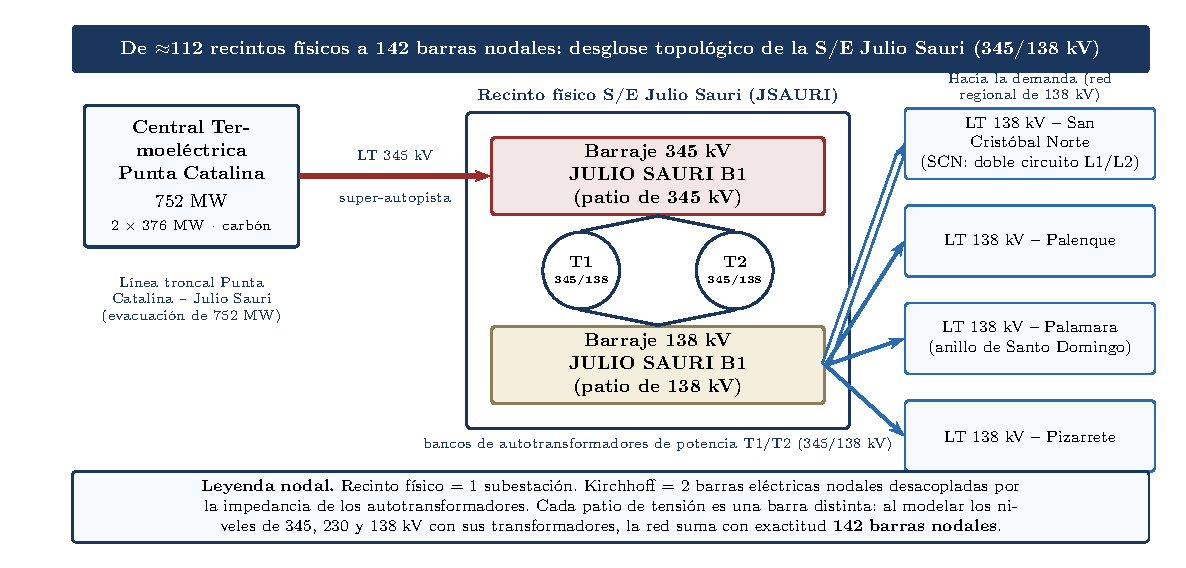
\includegraphics[width=0.78\textwidth]{fig_diagrama_1_jsauri_345_138.pdf}
\caption{Kirchhoff decoupling at the Julio Sauri 345/138 kV substation. The 345 kV super-highway that evacuates the Punta Catalina complex ($2 \times 376$ MW) terminates in its own yard, decoupled by the impedance of the T1/T2 autotransformer banks from the regional 138 kV yard that feeds the San Crist\'obal corridor and the metropolitan ring. Wherever a transformation exists, the fenced estate yields two buses; modeled across all voltage strata, the network totals exactly 142 nodal buses.}
\label{fig:jsauri}
\end{figure*}

\subsection{The bulk strata and the metropolitan 138 kV ring}
\label{sub:strata}

Three strategic substations articulate the grid: \textbf{JSAURI} (345/138~kV, system slack at $V = 1.02\ \mathrm{pu}$, receiving Punta Catalina's $2 \times 376 = 752$~MW coal generation); \textbf{PALA} (metropolitan load center, 1,645~MW demand with three 10.77~MW local backup units); and \textbf{SCN} (southwestern renewable hub: 58.9~MW hydro, 95~MW solar, 34~MW wind). Modular decarbonization testbed assets (a 50~MW PEM electrolyzer and 1,400~MW modular PWR units across JSAURI and SCN) are non-operational, excluded from the installed capacity (\texttt{in\_service = false} in \texttt{seni\_real\_base}), preserving operational fidelity while providing transition benchmark readiness. The metropolitan Ozama region consumes $>40\%$ of national demand, served via the geometric redundancy of the JSAURI--PALA--SCN 138~kV triangle (corridors of 70.5~km, 22.1~km, and 30.86~km, reinforced by a 230~kV tie). The loss of any single circuit is absorbed by surviving paths, satisfying the $N-1$ resilience criteria evaluated in Part~II~\cite{seni142part2}.

The 1,645~MW demand at PALA represents the aggregate load center of the metropolitan macro-domain, distributed across 28 metropolitan 138~kV substations (no single bus exceeding 120~MW), supported by $\approx 250$~MW of local generation. At the 3,450~MW national peak state, the reported inter-domain transfers across the four Law 368-22 macro-domains are: $\Omega_{\mathrm{Metro}}$ imports a net 1,395~MW across border set $\Gamma$; $\Omega_{\mathrm{Sur}}$ exports $+930$~MW (Punta Catalina and hydro); $\Omega_{\mathrm{Este}}$ exports $+420$~MW (Quisqueya, AES Andr\'es); and $\Omega_{\mathrm{Norte}}$ maintains local balance. The metropolitan import is carried by 345, 230, and 138~kV corridors totaling $>2,200$~MVA capacity at 63--72\% peak loading, ensuring post-contingency thermal compliance under all $N-1$ conditions (Part~II~\cite{seni142part2}).

\subsection{Ten sovereign territorial microgrids}
\label{sub:microgrids}

Law 368-22 organizes the national territory into ten planning regions; the benchmark adopts them as its ten territorial microgrids and bundles them, for numerical condensation, into the four electrical macro-subdomains of the HBCF. The mapping and the representative anchors of each region as they appear in the operational record are listed in the released dataset.

Figure~\ref{fig:hbcf_schur} displays the resulting diakoptic map: four macro-subdomains $\Omega$ over the insular geography, the trunk borders $\Gamma$ (the 230/138~kV ties cut by Kron reduction), and the silicon key performance indicators of the condensed solve. Numerically, the partition assigns the 112 interior buses to the four macro-subdomains as $\mathbf{A} = \operatorname{diag}(18, 28, 23, 43)$ (Metropolitan, South, East, North), closed by a minimal boundary $\Gamma$ of 30 buses ($112 + 30 = 142$ nodal buses).

% ---- Figure 4 injection block (verbatim from the sealed master;
%      resolved through \graphicspath{{figuras/}} in the host preamble) ----
\begin{figure*}[!t]
\centering
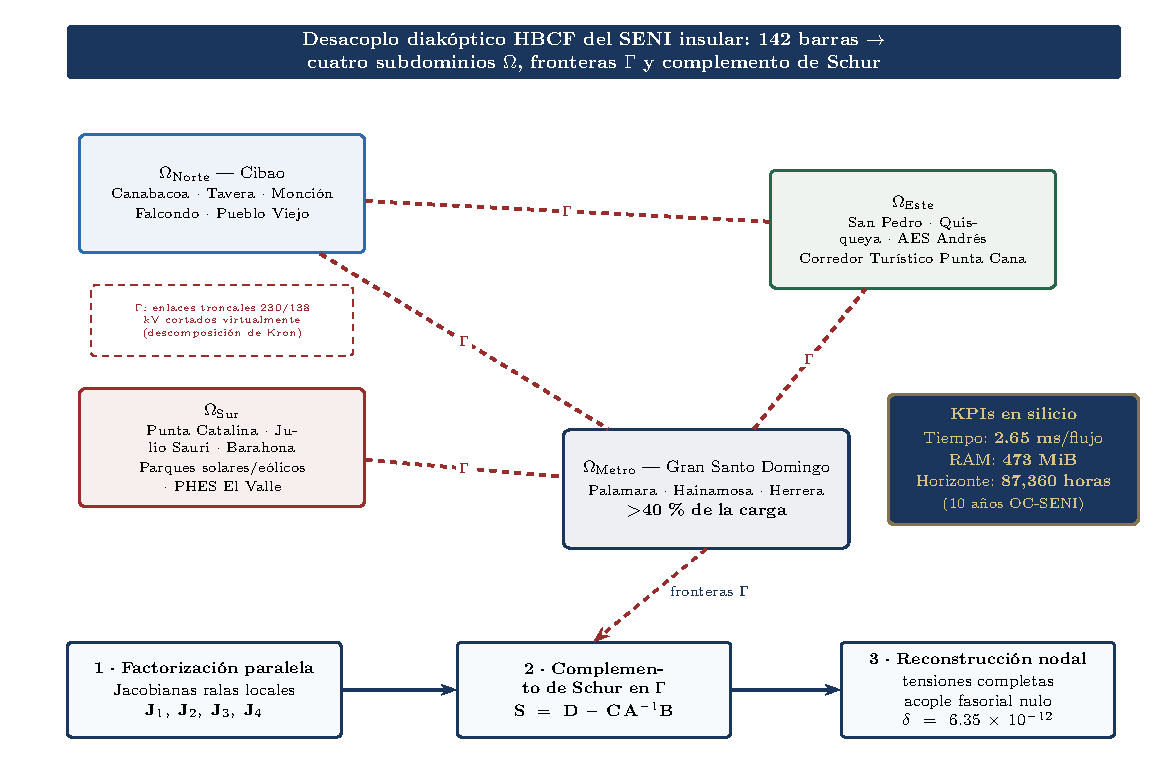
\includegraphics[width=0.75\textwidth]{fig_diagrama_2_schur_hbcf.pdf}
\caption{Spatial HBCF diakoptic partitioning of the insular grid. The ten territorial microgrids of Law 368-22 bundle into four electrical macro-subdomains $\Omega$ (North/Cibao, South, East, Metropolitan); only the trunk borders $\Gamma$ --- the 230/138 kV ties cut by Kron reduction --- travel to the Schur complement $\mathbf{S} = \mathbf{D} - \mathbf{C}\mathbf{A}^{-1}\mathbf{B}$, with block structure $\mathbf{A}, \mathbf{B}, \mathbf{C}, \mathbf{D}$ over the interior/border ordering. Silicon key performance indicators: 2.65 ms per national AC state, 473 MiB resident, over the standardized horizon of 520 complete weekly cycles (87,360 h; OC-SENI telemetry), with fasorial border-coupling residual $\delta = 2.788 \times 10^{-14}$ pu.}
\label{fig:hbcf_schur}
\end{figure*}

\subsection{Data provenance and the boundary-state manifest}
\label{sub:provenance}

Physical substation footprints, topological bus connections, and geographical corridor
trajectories are derived directly from the official single-line CAD blueprints maintained by the
transmission system operator (ETED). The associated branch electrical parameters
($R$, $X$, $B$, and MVA thermal ratings) and operational baseline setpoints are adopted from the
official OC-SENI and ETED reference system datasets \cite{ocseni}, \cite{eted}, structured under
the Common Information Model (CIM) conventions of IEC 61970 \cite{iec61970}. Power-quality-relevant
quantities follow the measurement definitions of IEC 61000-4-30 \cite{iec61000} and IEEE Std 1459
\cite{ieee1459}. Every coupling term reaching the master solver --- the $(P_g, Q_g)$ injections of the flexibility constellation of Part~II~\cite{seni142part2} --- travels through a boundary-state manifest chained and signed with SHA-512. Provenance thus runs unbroken from operator archives \cite{ocseni}, \cite{eted} to solver input to published figures --- guaranteeing reproducible verification.

\subsection{The synthetic canon versus the measured island}
\label{sub:canon}

The contrast between SENI-142 and synthetic benchmarks centers on two empirical axes: \emph{temporal depth} and \emph{consequence}. Synthetic cases provide static, idealized snapshots; SENI-142 supplies 87,360 consecutive hourly states across 520 complete weeks (2016--2025 archive), enabling hypothesis testing against realized weather, demand, and dispatch. Furthermore, while synthetic networks carry no real-world operating histories, every SENI trunk corridor reflects documented outage logs, maintenance records, and contingency events under insular operating conditions.

% ---- Table II (verbatim content of the sealed master) ----

% =========================================================================
% p1_sec08_conclusion.tex — Part I conclusion, structural nomenclature.
% =========================================================================
\section{Conclusion and Outlook of Part~I}
\label{sec:conclusion}

This Part~I of the SENI-142 study contributed the open structural layer of a measured national transmission benchmark: an open-access, georeferenced model of the Dominican bulk grid --- 142 nodal buses (115 bulk buses and 27 retained 69~kV boundary ports derived from 112 substation estates), 135 lines, 58 transformers, and ten territorial microgrids under Law 368-22 --- released with complete parameters, provenance, and validation harness via GitHub. The HBCF diakoptic partition into four macro-subdomains admits an exact Schur condensation with complexity $O(\sum_k N_k^3 + N_B^3)$ and a measured algebraic residual $\delta = 2.788 \times 10^{-14}\ \mathrm{pu}$. A four-phase fail-closed digital-twin lifecycle with detached SHA-512 custody guarantees determinism: the data verifier passes 41/41 checks, and the published mutation suite is detected 12/12 under canonical corruptions with a passing control. The resilience layer formalizes the operator's 215-contingency catalog under an explicit two-layer reserve doctrine and a four-clause static PASS battery.

Two research routes follow at the structural level: (i) \textbf{physics-informed neural surrogates} trained on the released hourly horizon with exact AC solvers as falsification oracles \cite{misyris2020}; and (ii) \textbf{grid-forming EMT co-simulation} embedding converter dynamics \cite{rosso2021}, \cite{ieee2800} to investigate frequency formation. The companion Part~II~\cite{seni142part2} completes the study with the multi-vector flexibility layer, the 87,360-state campaign, severe common-mode contingencies, and insular policy implications.


\noindent\textbf{Data Availability.}~The SENI-142 dataset, network parameters, validation harness, and sealed resilience record are openly available at \url{https://github.com/Junvillan/seni142-benchmark} and archived under DOI:~\href{https://doi.org/10.5281/zenodo.23484704}{10.5281/zenodo.23484704}. High-resolution vector figures are available and resolved via the repository's \texttt{figuras/} directory. The release ships the data-driven verifier \texttt{verify\_seni142\_benchmark.py}, which re-derives every sealed quantity of the release from the canonical CSV/NPZ bundle --- 41/41 checks PASS (bus and branch censuses, peak load, unique slack, block-diagonal Schur structure, and the eight contingency balances).


\section*{Acknowledgment}
The author dedicates this work to the memory of Eng.~Arturo Lamarche (E.P.D., in memoriam)---an esteemed mentor, master of Dominican power systems, and tireless guardian of the national grid. His lifelong devotion, technical rigor, and unwavering vigilance over the integrity of the Dominican electrical system during the pivotal expansion of the 345/138\,kV bulk network left an indelible mark on generations of electrical engineers. His legacy endures in every bus, corridor, and protective boundary analyzed in this benchmark.


\bibliographystyle{IEEEtran}
\bibliography{referencias}

\end{document}
